\documentclass[xcolor=svgnames,aspectratio=169]{beamer}

\usetheme{Boadilla}
\useoutertheme[subsection=false]{smoothbars}
\usefonttheme{serif}
\usecolortheme{seagull} % dove fly seagull
\useinnertheme{rounded}
\usepackage{pifont}
\usepackage{time}       % date and time
\usepackage{url}
\usepackage{graphicx}
\usepackage[T1]{fontenc}    % european characters
% \usepackage{pgothic}
\usepackage{yfonts}
% \usepackage{courier}
\usepackage{amssymb,amsmath}  % use mathematical symbols
\usepackage{palatino}      % use palatino as the default font
\usepackage{listings}   % insert python code into presentation
\usepackage{multirow}
\setbeamercovered{transparent}
\setbeamertemplate{itemize subitem}[triangle]
\setbeamertemplate{navigation symbols}{}

\newcommand{\tc}{\textcolor}
\newcommand{\select}{$\leadsto~$}
\newcommand{\fb}{\framebox}
\def\ra{$\rightarrow$\,\,}
\definecolor{cadet}{rgb}{0.33, 0.41, 0.47}
\newcommand{\hi}[1]{{\color{cadet}\textsl{#1}}}
\newcommand{\chacha}[1]{\centering{\scalebox{2}{\fontsize{12pt}{0pt}\normalfont{#1}}}}
\newcommand{\chapter}[1]{\begin{frame}{}\chacha{#1}\end{frame}}
\newcommand{\chapterDouble}[2]{\begin{frame}{}\chacha{#1}\\\medskip\chacha{#2}\end{frame}}
\newcommand{\resetEnv}{
  \colorlet{structure}{mystruct}
  \beamertemplateshadingbackground{blue!5}{gray!10}
  \beamertemplateshadingbackground{white}{white}
}
\usepackage{mathtools}
\usepackage{xcolor}
\usepackage{verbatim}
\usepackage{listings}
\usepackage{keystroke}

\definecolor{byzantium}{rgb}{0.44, 0.16, 0.39}
\definecolor{ferrariRed}{rgb}{1.0, 0.11, 0.0}

% tiny-scriptsize-footnotesize-small-normalsize-large-Large-LARGE-huge-Huge

\begin{document}

\title[VisIt Workshop]{\LARGE Parallel programming in Chapel}
\author[]{{\large\sc Juan Zuniga}\\{\small juan.zuniga@usask.ca}\\\bigskip {\large\sc Alex
    Razoumov}\\{\small alex.razoumov@westgrid.ca}}
\date[May 2017]{\textcolor{byzantium}{\footnotesize slides and code examples at at ...}}
\institute[]{\includegraphics[width=0.25\columnwidth]{./logos/ccLogo}
  \hspace{.65cm}\includegraphics[width=0.35\columnwidth]{./logos/WG-Logo-Jan16}}

\begin{frame}
  \titlepage
\end{frame}

\section{Intro}
\subsection{} % creates page markers at the top

\newcommand{\tnij}{\ensuremath{T^{(n)}_{i,j}}}

\begin{frame}{}
  \begin{itemize}\setlength{\itemsep}{3mm}
    \item Simple 2D heat (diffusion) equation
    \[
      {\partial T(x,y,t)\over\partial t}={\partial^2 T\over\partial x^2}+{\partial^2 T\over\partial y^2}
    \]
    {\footnotesize
      \item Discretize the solution $T(x,y,t)\approx T^{(n)}_{i,j}$ with $i=1,...,n$ and $j=1,...,n$
      \item Imagine a metallic plate being constantly heated in one corner, e.g. $T^{(n)}_{1,1}=1$
      \item Everywhere else the initial solution is $T^{(0)}_{i,j}=0$}
    \item Discretize the equation with forward Euler time stepping
    \[
      {T^{(n+1)}_{i,j}-\tnij\over\Delta t}=
      {T^{(n)}_{i+1,j}-2T^{(n)}_{i,j}+T^{(n)}_{i-1,j}\over(\Delta x)^2}+
      {T^{(n)}_{i,j+1}-2T^{(n)}_{i,j}+T^{(n)}_{i,j-1}\over(\Delta y)^2}
    \]
  \end{itemize}
\end{frame}

\begin{frame}{}
  \begin{itemize}\setlength{\itemsep}{3mm}
    \item For simplicity assume $\Delta x=\Delta y=1$
    \item Use $\Delta t=1/4$ which is the upper limit of numerical stability
    \item The finite difference equation becomes
    \[
      T^{(n+1)}_{i,j} = {1\over4}\left[T^{(n)}_{i+1,j}+T^{(n)}_{i-1,j}+T^{(n)}_{i,j+1}+T^{(n)}_{i,j-1}\right]
    \]
    \item The objective is to find $T_{i,j}$ after a
    certain number of iterations, or when the system is in steady state)
    \item Once done, also try increasing the number of points in the grid to illustrate the advantage of
    parallelism
  \end{itemize}
\end{frame}

% language syntax and the compiler, the notions of locality and parallelism and how they are orthogonal
% concepts in Chapel

\section{Chapel base language}
\chapter{Chapel base language}
\subsection{} % creates page markers at the top

\begin{frame}{Why another language?}{\url{http://chapel.cray.com}}
  \begin{itemize}\setlength{\itemsep}{1mm}
    \item Shared- and distributed-memory parallelism intrinsic part of the language
    \item Much higher-level (and much easier to use!) than MPI
    \medskip
    \begin{itemize}\setlength{\itemsep}{1mm}
      \item ``Python for parallel programming''
      \item few lines of Chapel code typically replace $\sim$100 lines of MPI code
    \end{itemize}    
    \item Focus on performance
    \medskip
    \begin{itemize}\setlength{\itemsep}{1mm}
      \item simple Chapel codes perform as well as optimized C/C++/F90 code
      \item very complex Chapel codes run at $\sim$70\% performance of a similar well-tuned MPI code (not
      bad in my opinion, but room to improve)
    \end{itemize}    
    \item Perfect language for learning parallel programming for beginners
    \item Open-source: can compile on all Unix-type platforms, precompiled for MacOS
    \item Chicken-and-egg situation: too few people know/use Chapel ~$\Longleftrightarrow$~ too few HPC
    centers install and promote it
  \end{itemize}
\end{frame}

\begin{frame}{Brief history}
\end{frame}

\begin{frame}{Useful links}
  \begin{itemize}\setlength{\itemsep}{3mm}
    \item Getting started guide for Python programmers
    {\small\url{http://chapel-for-python-programmers.readthedocs.io/basics.html}}
    \item Data parallelism in Chapel \url{http://chapel.cray.com/tutorials/ACCU2017/03-DataPar.pdf}
    \item Short tutorial from David Bunde \url{http://faculty.knox.edu/dbunde/teaching/chapel}
    \item docs and examples for various Chapel modules in \texttt{\$CHPL\_HOME/modules/}, e.g.,
    \texttt{standard/} or \texttt{dists/}
    \item \url{https://learnxinyminutes.com/docs/chapel}
    \item \url{https://stackoverflow.com/questions/tagged/chapel}
  \end{itemize}
\end{frame}

\begin{frame}{Exercise: using functions and control flow}
  Write a Chapel code to find the root of the equation $x^5 + 8x^3 - 2x^2 + 5x - 1.2 = 0$ using the bisection
  method in the interval [-1,1]
  \begin{columns}[]
    \column{0.45\textwidth}
    \begin{itemize}\setlength{\itemsep}{3mm}
      \item Calculate the function at the ends and the midpoint of the interval
      \item Depending on the signs of the three computed values, let the midpoint be either the new left
      or the new right end
      \item Repeat until your error is below $\Delta x=10^{-8}$
    \end{itemize}
    \column{0.55\textwidth}
    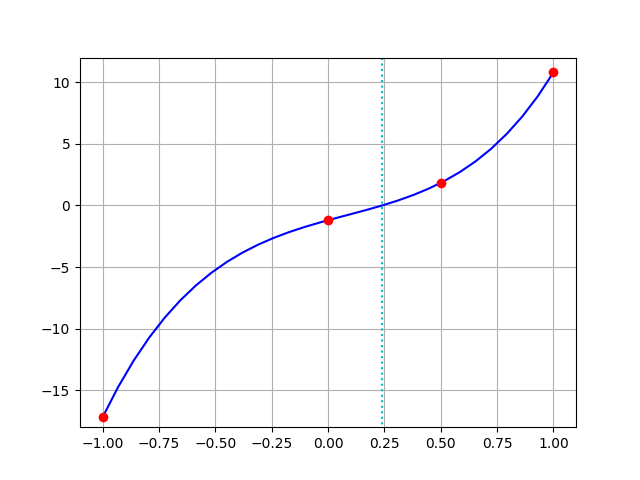
\includegraphics[width=0.95\columnwidth]{figs/bisection.png}
  \end{columns}
\end{frame}

% forall and coforall in abstract level

\section{Task parallelism}
\chapter{Task parallelism}
\subsection{} % creates page markers at the top

% revisiting the notion of locality, where in the hardware the tasks (or the different locales) are
% running, parallel data structures, domain maps

\section{Data parallelism}
\chapter{Data parallelism}
\subsection{} % creates page markers at the top

\begin{frame}{}
  \begin{itemize}\setlength{\itemsep}{3mm}
    \item domain types \url{http://chapel.cray.com/tutorials/ACCU2017/03-DataPar.pdf}
    \item two
  \end{itemize}
\end{frame}


% http://chapel.cray.com/docs/1.14/primers/primers/distributions.html
% http://chapel.cray.com/tutorials/ACCU2017/03-DataPar.pdf
% builtin Locales variable
% - for loc in Locales {} followed by on loc {}
% - do something on Locales[1]
% become very proficient with regular domains
% blocks.chpl
% - introduce a block-distributed domain and an array of to of it
% cyclic.chpl
% evolution.chpl
% periodic.chpl
% - exercise: modify evolution.chpl to put in periodic BCs
% - check energy conservation
% - write out each timestep to an ASCII file

% iterators, I/O files, modules and other packages?
% how to call C/C++/Fortran functions from Chapel, especially popular numerical libraries

\section{Advanced language features}
\chapter{Advanced language features}
\subsection{} % creates page markers at the top

\begin{frame}{}
  \begin{itemize}\setlength{\itemsep}{3mm}
    \item one
    \item two
  \end{itemize}
\end{frame}

\section{Summary}
\subsection{} % creates page markers at the top

\begin{frame}{}
  \begin{itemize}\setlength{\itemsep}{3mm}
    \item one
    \item two
  \end{itemize}
\end{frame}


\end{document}

Use the 2D diffusion problem to show all Chapel features:

part 1:
a. base language: define T as a 2D array, and compute its elements one by one with nested for loops
b. Task parallelism 1: substitute for loops with forall loops.
c. Task parallelism 2: decompose T in sub-matrices and distribute them with a coforall loop

part 2:
d. Data parallelism: work with T as a matrix, explore mapping its domain with different methods.
e. Advanced features: Save data of iterations to file, maybe create a customized iterator for the problem ?
